\documentclass[12pt,a4paper]{article}
\usepackage[utf8]{inputenc}
\usepackage[text={17cm,25.5cm},centering]{geometry}
\usepackage{tikz}
\usepackage{float}
\usepackage{listings}
\usepackage{multicol}
\usepackage{color}
\usepackage{minibox}
\definecolor{red}{rgb}{1.0,0.7,0.7}
\definecolor{green}{rgb}{0.7,1.0,0.7}
\definecolor{blue}{rgb}{0.8,0.9,0.9}
\usetikzlibrary{arrows,calc}
\tikzset{
%Define standard arrow tip
>=stealth',
%Define style for different line styles
connection/.style={thick, dotted},
}
\lstset{
  basicstyle=\footnotesize,
  numbers=left,
  escapechar=`
}

\title{Bringing COP to embedded programming}
\author{Mikhail Afanasov}

\begin{document}

\maketitle

\paragraph{Abstract.} Wireless Sensor Networks (WSNs) are widely applied in different areas, such as health monitoring, wildlife tracking, smart home etc. These days WSNs are used in highly changing environments and the software for WSNs needs to be adaptable but still simple. 

Context-oriented programming (COP) is a programming technique which makes it possible to create an adaptive software. Such a software could adapt to changes in the environment and to evolve according to this changes. The term ``evolve'' means that software can change behavior and this behavior depends on the context in which it is executed. This technique could simplify the complex source-code for WSNs.

In this work we review existing applications of WSN and discuss how COP could be applied to the different scenarios. We also propose methods like context classification, context events and context rules to simplify programming for WSNs.

\section{Introduction}
\paragraph{}
WSNs are often deployed in a highly changing environment. It  means that a programmer should always care about changes in data acquired by sensors. It leads to increasingly complex source-code. This problem has more significance in mobile WSNs, where we should be aware of location changes. Thus it is hard to implement and maintain such a software. Bringing Context-Oriented Programming in programming for WSN could solve the problem.

Context-Oriented Programming (COP) \cite{hirschfeld08} is an approach which provides an opportunity for a programmer to develop a software which can dynamically change the behavior depending on context conditions. Context can be defined as ``any information that can be used to characterize the situation of an entity, where an entity can be a person, place or physical object" \cite{dey99}. Context-awareness can be defined as detecting current internal or external state of WSNs.

The context structure for WSNs could be very complex and have nontrivial interaction. But contexts can be divided into groups and considered as classes of contexts. Such classification brings COP on a new level of abstraction and makes it possible to operate complex structures of contexts as a superposition of smaller substructures. It also simplify the integration between different platforms, since another platform could be considered as a new class.

In this work context transition in WSNs are also considered. WSNs should be aware not only of the context, but also of the transition between contexts. In other words, system should perform particular actions in the same time when context is changed. It could be done by providing \textit{context transition behavior}. Thus programmer can specify particular behavior of WSN when context transition occurred. Programmer should also be able to define restrictions and dependencies in context transitions. During the execution there are contexts, which can not be activated while another context is active. If context has dependencies, then it can not be activated while another contexts is deactivated. Context restrictions and context dependency could clarify complex interactions between contexts.

In this work we propose possible solutions of the problems stated above. We review several scenarios of using WSNs and propose how COP can be used in these scenarios. For every scenario we show a context structure and classification, and describe behavior of the WSN. At the end of the paper we discuss possible ways to manage context transitions and restrictions. We also show an implementation of COP using one of the languages for programming for WSNs.

\section{Scenarios}\label{sec:scn}
\paragraph{}
WSNs are systems in which numerous tiny sensing devices are distributed over the environment to study it. They are proposed in many engineering, scientific,  civil and military applications and widely used to monitor different entities in areas ranging from wildlife \cite{juang02} \cite{lingren08} \cite{pastor08} to human health-care \cite{lorincz09} \cite{alemdar10}. Some of them are discussed in this paper.
\subsection{Wildlife tracking.} In biology research there is a necessity to track wildlife. For example, WSN devices can be attached to wildlife species ( e.g. zebras \cite{juang02}, badgers \cite{dyo09} or turtles \cite{gorlick07}) to study their behavior. Human intervention is highly undesirable in this kind of research \cite{juang02}, that is why WSNs are very well suited there.

\paragraph{Community class.} Usually the monitored area extends beyond the communication range of nodes. Thus, the network is characterized by intermittent connectivity among nodes \cite{lukac06}. But animals are social beings, so it is possible to explore recognizable patterns of movement and community interaction \cite{pastor08}. We can detect a group of nodes which is representing a separate community and assume that \textit{community} is a context. An event when node leaving the group or joining to the group could be considered as a change of the context.

\paragraph{Base station class.} In the most of WSNs the main goal is to acquire the data from the nodes and to deliver it to the base station. Because of the wide area of monitoring, nodes are not always in the range of the base station. So, it is possible to extract another context \textit{base station}. It is activated when the base station is in the communication range and deactivated when it's not.

\paragraph{Activity class.} Species' activity can be characterized by several states such as: sleeping, rest and movement \cite{juang02}. Thereby, we can emphasize \textit{sleeping} (specie isn't moving), \textit{rest} (specie is moving for a short distances) and \textit{movement} (specie is moving for a long distances) contexts.

\paragraph{Battery level class} Another aspect of WSNs is power consumption. During the execution we can track the battery level. Within the  \textit{low battery level} context node could switch off sensors with low priority.

\paragraph{}
Contexts' diagram for wildlife tracking scenario is displayed on the figure \ref{fig:wtd}. Contexts described above can be separated into different classes: \textit{Community class}, \textit{Base station class}, \textit{Activity class} and \textit{Battery level class}. \textit{Community class} indicates whether the node is belonged to the particular community or not. \textit{Base station class} consist of two contexts \textit{Within the BS range} and \textit{Out of BS range}. \textit{Activity class} contains possible activities of specie. \textit{Battery level class} includes \textit{Low level}, \textit{Normal level} and \textit{High level}. Within the separate class contexts transactions can be performed independently. However, there are could be restrictions for contexts' transactions. For example, we could not expect dramatic changes in network topology, while \textit{sleep} context is activated. Thus, within \textit{Community} and \textit{Base station} classes there are transition condition: if \textit{sleep} context is deactivated, then it is possible to perform transaction within classes mentioned above. Another restriction is a battery level. Context \textit{Within the base station} could be activated only when the node has sufficient battery level, i.e. \textit{High level} or \textit{Normal level} are activated.

While particular transactions between contexts are performed, a node should switch some sensors on or off. For example, if \textit{Within BS range} context is activated, then the node should switch on high range transmitter, but switch it off if \textit{Out BS range} is activated. While \textit{sleep} context is activated, GPS sensor should be switched off. While \textit{low level} is activated, system have to disable sensors with low priority. Thus we should be able to define particular behavior for transactions between context.

\begin{figure}[H]
\centerline{
  \includegraphics{wildlifetracking.png}
}
\caption{Diagram of the contexts for wildlife tracking.}
\label{fig:wtd}
\end{figure}

\subsection{Healthcare}\label{healthcare}
\paragraph{}
Another scenario of WSNs application is healthcare industries. Medical applications of WSNs would improve the existing healthcare and especially for children, elderly and ill. This kind of WSNs should not only provide sensed data, but also identify current condition of the person, in other worlds, identify the context. The context information helps in understanding current condition and taking the situation under control.
Context-awareness, defined as ``providing relevant information and/or services to the user, where relevancy depends on user's task \cite{dey99-1}", is a main issue for the health monitoring \cite{ng04}. Depends on tasks, such as: activities of daily living monitoring, fall and movement detection, local tracking, medication intake monitoring, and medical status monitoring \cite{alemdar10}, we can extract possible contexts.

\paragraph{Emergency class.} \textit{Emergency} class implies, but not limited to, such events as: falling, heart attack, critical health condition etc. In case of emergency software activates additional sensors to get more precise information about an event. For example, in case of falling or heart attack, GPS sensor could be activated and emergency message could be sent to appropriate services.

\paragraph{Activity class.} This group of contexts consists of such activities as: walking, sitting, laying etc. Usually, if a person is sitting or laying, then sudden falling is not expected. And if \textit{walking} context is activated, software can switch on GPS tracker and try to detect sudden falling by an accelerometer sensor. Software could also track unusual activities. For example, if a person is \textit{sleeping} too long, then \textit{emergency} context could be activated. 

\paragraph{Location class.} It includes \textit{indoor} and \textit{outdoor} contexts. While GPS works well outdoor and could be used to help people with cognitive disabilities or to identify person's location in emergency situation, it does not works properly indoor \cite{alemdar10}. Activation of \textit{indoor} context will force software to use another ways to detect person's location. For example, by using Radio Frequency Identification (RFID) markers \cite{chang08}.

\paragraph{}
Figure \ref{fig:hcd} displays the diagram for possible healthcare contexts. Here \textit{Emergency}, \textit{Activity} and \textit{Location} contexts classes can be highlighted. \textit{Location} class contains \textit{indoor} and \textit{outdoor} contexts. We have to define conditions of contexts transition and behavior during these transitions. Thus, while \textit{indoor} context is active, GPS should be switched off. \textit{Outdoor} context can not be activated while \textit{sleep} context is active. But, if it is activated, then we should enable GPS. \textit{Emergency} class consist of \textit{normal} context, \textit{critical condition}, \textit{falling} and \textit{heart attack}. \textit{Normal} context represents a normal state, but if sensors detects emergency situation like \textit{critical condition}, \textit{falling} or \textit{heart attack}, corresponding context is activated. But \textit{falling} context can not be activated, while \textit{sleeping} context is active. \textit{Activity} class includes contexts \textit{idle}, \textit{moving}, \textit{sitting} and \textit{sleeping}. There are also restrictions: system can not perform a transition from \textit{sleeping} contexts to the \textit{moving} context directly. \textit{Sleeping} context can not be activated while \textit{outdoor} context is active. But if \textit{sleeping} context is activated, system should disable accelerometer sensor, since we can not expect sudden falling. While \textit{moving} \textit{outdoor}, GPS sensor should be activated for precise location tracking.

\begin{figure}[H]
\centerline{
  \includegraphics{healthcare.png}
}
\caption{State machine for healthcare contexts.}
\label{fig:hcd}
\end{figure}

\subsection{Smart home}
\paragraph{}
Humans' life quality could be dramatically increased by using WSNs to build a \textit{Smart Home}. In this scenario WSNs is embedded to the house or a flat to detect current conditions of householders and the environment.

\paragraph{Emergency class.} This class is very similar to the \textit{emergency} class discussed in \ref{healthcare}. If WSN detects fire or housebreaking it can send an emergency call. If integrated with \textit{Healthcare system}, it can also activate emergency depends on \textit{Healthcare system} context. For example, if a householder has an injury or heart attack, the WSN can also activate a context from \textit{emergency} class.

\paragraph{Householder's location.} WSN can also track a householder's location. For example, if a householder moves from a kitchen to a dining room, the system switches off the light in the kitchen and switches on the light in the dining room. In this context system is also able to detect housebreaking. For example, if an unrecognized person appears in the house, while a householder is sleeping, then WSN activates the \textit{emergency} context. If a householder leaves the house, then \textit{Smart Home} could just lock the door. If a householder is nearby, then it could open the door.

\paragraph{Health monitoring.} WSN can be programmed to detect specific conditions and activate a specific context. For example, if the temperature in the room is lower (or higher) than normal, system can enable air heating (or conditioning) to return the temperature to the normal state. If \textit{Healthcare System} is integrated to \textit{Smart Home}, so the system can notify the householder about his current condition and recommend activities to improve householder's state of health.

\paragraph{}
Figure \ref{fig:shd} shows a state diagram of possible contexts of \textit{Smart Home}. In this application three classes could be found: \textit{Emergency} class, \textit{Location} class and \textit{Climate} class. Contexts of \textit{Emergency} class are activated if system detects intruders, fire or health emergency. There is a necessity to perform particular actions during context transition. For example, to call the police, the fire or an ambulance. \textit{Location} class includes \textit{outdoor} and rooms in house. During context transitions within \textit{location} class, system have to turn on/off lights and lock/unlock door. \textit{Climate} class could contains temperature contexts. If system detects high or low temperature, then it enables conditioner or heater.

\begin{figure}[H]
\centerline{
  \includegraphics{smarthome.png}
}
\caption{A state diagram for smarthome.}
\label{fig:shd}
\end{figure}

\section{Context Recognition}
\paragraph{}
Regardless the scenario, we can emphasize several context detection mechanisms. The first step of context recognition is acquiring the low-level sensor readings. Considering these readings, we can then extract the context \cite{korel10}.
\paragraph{Context-Aware Packets}method allows single sensor to share sensed data in order to detect meaningful context model from manifold inputs \cite{michahelles02}. This mechanism assumes that every node can send a packet with data acquired by node to the base station. Base station then analyzes the data and recognizes the context.
\paragraph{Artificial Neural Networks}(ANNs) method is used as a solid clustering algorithm for context-awareness in sensor networks \cite{korel10}. The low-level sensors produce a noise while acquiring the data. While ANNs still perform well despite of nose, they also add a new context to the system without intervention from a user.
\paragraph{Bayesian Networks}(BNs) method makes it possible to estimate current context statistically \cite{korel10}. It relies on the intensity of the sensing data. The higher the intensity, the more significant the data is.

\section{Discussion}
\paragraph{}
Most of the implementations of WSNs consider that context is managed by human or by program on a remote computer or a base station, but there are cases when wireless nodes should manage the context by themselves. For example, in wildlife tracking nodes could be out the range of the base station for a long time, but it is still necessary to manage the context.

While global contexts are described, we need to create tools to manage the context on a low hardware level, like wireless sensor node. We didn't consider decision making process, but focused on managing the behavior within the given context. In a trivial case, programmer activates context manually within the program.

As was considered in a previous sections, different context and context classes (groups) can be extracted in different scenarios. There are also actions should be performed before activation and after deactivation of the context. Each context also has transition rules, i.e. transition from one context to another can be performed if it satisfies the particular conditions.

According to scenarios described in the section \ref{sec:scn}, four types of constructs should be defined: \textit{context event}, \textit{context transition}, \textit{check} and \textit{trigger}. \textit{Context event} occurs if sensed data satisfies one of the conditions. \textit{Context transition} is the fact of the transitions between contexts and treated as an \textit{event}. \textit{Trigger} is a condition which triggers the transition between contexts, \textit{check} verifies if the transition is possible or not. In other words, we have two types of events and two types of transitions rules. In the figure \ref{fig:enr} different combinations of rules and events are shown. Thus, \textit{context event} (or sensed data) as well as \textit{context transition} can \textit{trigger} the transition between contexts. But we also need to verify validity of such a transition. So we can use \textit{context event} and \textit{context transition} as \textit{checks}. In other words, transition can be performed only if another \textit{context transition} has been performed or if another \textit{context event} has been occurred.

\begin{figure}[H]
\centerline{
  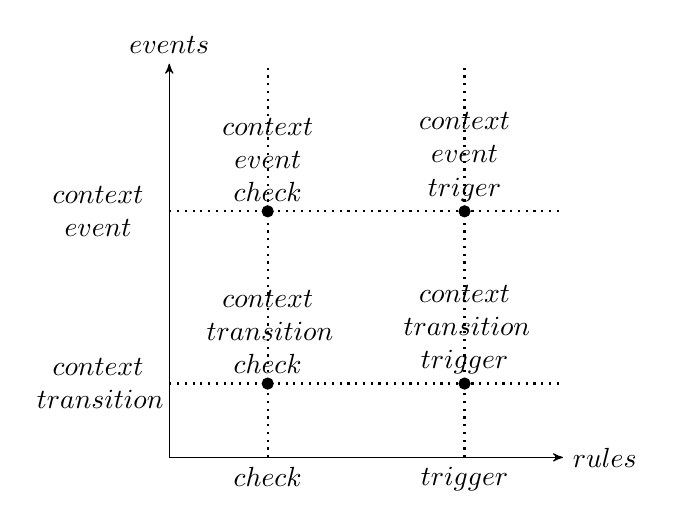
\begin{tikzpicture}[scale=1]
    % Axis
    \coordinate (y) at (0,5);
    \coordinate (x) at (5,0);
    \draw[<->] (y) node[above] {$events$} -- (0,0) --  (x) node[right] {$rules$};
    \draw[connection] let \p1=(0, .9375), \p2=(5, .9375) in (0,\y1) node[left, text width=1.55cm,align=center] {$context$\\$transition$} -- (\x2, \y1);
    \draw[connection] let \p1=(0, 3.125), \p2=(5, 3.125) in (0,\y1) node[left, text width=1.55cm,align=center] {$context$\\$event$} -- (\x2, \y1);
    \draw[connection] let \p1=(1.25, 0), \p2=(1.25, 5) in (\x1, 0) node[below, text width=1.55cm,align=center] {$check$} -- (\x1, \y2);
    \draw[connection] let \p1=(3.75, 0), \p2=(3.75, 5) in (\x1, 0) node[below, text width=1.55cm,align=center] {$trigger$} -- (\x1, \y2);
    \filldraw [black] (3.75, .9375) circle (2pt) node[above, black, text width=1.55cm,align=center] {$context$ $transition$\\$trigger$};
    \filldraw [black] (1.25, .9375) circle (2pt) node[above, black, text width=1.55cm,align=center] {$context$ $transition$\\$check$};
    \filldraw [black] (1.25, 3.125) circle (2pt) node[above, black, text width=1.55cm,align=center] {$context$ $event$\\$check$};
    \filldraw [black] (3.75, 3.125) circle (2pt) node[above, black, text width=1.55cm,align=center] {$context$ $event$\\$triger$};
  \end{tikzpicture}
}
\caption{Events and rules.}
\label{fig:enr}
\end{figure}

Context class can be considered as a state machine, where context is a state. In each scenario could be several state machines. Context transitions can be considered as changes of a state of the state machine. Context transitions have rules and constraints, thus state can not be changed if the conditions are not satisfied. Context transitions are initiated by triggers. There are also actions which should be performed before activation and after deactivation of the context. Thus, we can emphasize main requirements of the context-oriented language for embedded systems. Language should provide tools to:
\begin{itemize}
\item Define context
\item Define context-depended functions.
\item Define context configuration
\item Define actions before activation and after deactivation
\item Define rules of context activation
\item Define triggers
\end{itemize}

\section{Implementation}
\paragraph{}
We are using TinyOS and nesC language for demonstration purposes. In order to use context-oriented paradigm, we added new key-words in the language. We are also extended components by \textit{context} and \textit{context configuration}. \textit{Context} is an analog of \textit{module} and \textit{context configuration} is an analog of \textit{configuration}. These two components can be used as other components in nesC language.

\textit{Context} components is used to define context, possible transitions, actions before activation and after deactivation, layered functions, and to check transition conditions. In the rest it can be used like a \textit{module}.

\begin{figure}[H]
\begin{lstlisting}
context High {
  transitions Normal;
  uses interface Leds;
}
implementation {
  event void activated() {
  }
  event void deactivated() {
  }
  bool check() {
    return TRUE;
  }
  layered void toggle_leds() {
    call Leds.set(1);
  }
}
\end{lstlisting}
\caption{Context component.}
\label{fig:cc}
\end{figure}

On the figure \ref{fig:cc} context definition is displayed. Key word \textit{transitions} on the line 2 define legal transitions from context \textit{High}. It means, that only \textit{Normal} can be activated as the next context after \textit{High}. This definition is not mandatory. If \textit{transitions} are not defined, any transitions are legal. Line 3 represents regular nesC key word and means, that we are using \textit{Leds} component. Event \textit{activated} (line 6) is fired just before context activation, while event \textit{deactivated} (line 8) is fired just after deactivation. These events are also not mandatory. Method \textit{check()} represents \textit{context event check}. This method is called to verify conditions of context activation. If \textit{check()} returns FALSE, context will not be activated. If method is not defined, conditions will not be verified. Key-word \textit{layered} (line 13) indicates implementation of the function, which is specific for the current context. \textit{Layered} functions implementation is mandatory if they are defined in context configuration.

In the \textit{context} component \textit{context transition check} and \textit{context transition trigger} can also be specified. For example, on the line 2 (figure \ref{fig:ctre}) key-word \textit{while} declares, that transition from \textit{Indoor} to \textit{Outdoor} context can be activated only if \textit{Activity.Moving} context is active, where \textit{Activity} is a context class.

\begin{figure}[H]
\begin{lstlisting}
context Indoor {
  transitions Outdoor while Activity.Moving;
}
implementation {
}
\end{lstlisting}
\caption{Context transition rule example.}
\label{fig:ctre}
\end{figure}

Programmer can also specify \textit{Context transition trigger} within the \textit{context} declaration. For example, if we have integration between two WSNs \textit{Smart Home} and \textit{Health Care}, programmer may want to activate \textit{SamrtHome.Emergency} context if \textit{HealthCare.Emergency} context was activated. It can be done as it shown on the line 2 of the figure \ref{fig:ctre}.

\begin{figure}[H]
\begin{lstlisting}
context Emergency {
  triggers SmartHome.Emergency;
}
implementation {
}
\end{lstlisting}
\caption{Context transition trigger example.}
\label{fig:ctre}
\end{figure}

\textit{Context configuration} component is used to define layered functions and context configuration. In the rest it can be used like a regular \textit{configuration}.

\begin{figure}[H]
\begin{lstlisting}
context configuration Temperature {
  layered void toggle_leds();
}
implementation {
  contexts High,
    Normal is default,
    Low;
  components LedsC;
  High.Leds -> LedsC;
  Normal.Leds -> LedsC;
  Low.Leds -> LedsC;
  Error.Leds -> LedsC;
}
\end{lstlisting}
\caption{Context configuration component.}
\label{fig:ccc}
\end{figure}

In the listing \ref{fig:ccc} we assume, that contexts \textit{High}, \textit{Normal} and \textit{Low} are already defined. \textit{Error} context is default and generated by compiler, however it can be overridden by programmer in a standard context definition way. On the line 2 we declare a layered function, which should be implemented in each context. Lines 5, 6 and 7 show contexts belonging to the \textit{Temperature} class. It also indicates, that all declared contexts should implement layered functions. Line 6 also indicates that \textit{Normal} context will be active after initialization. The rest of the listing is a regular declaration of components and wires.

\textit{Context} and \textit{context configuration} has nesC-like structure and utilize the same logic. Both components can be used in native nesC way as a regular components.

\begin{figure}[H]
\begin{lstlisting}
module DemoC {
  uses context configuration Temperature;
  uses interface Boot;
}
implemetation {
  event vois Boot.booted() {
    activate Temperature.Low;
    call Temperature.toggle_leds();
  }
  event void Temperature.contextChanged(context_t con) {
  }
}
\end{lstlisting}
\caption{Components usage example.}
\label{fig:cue}
\end{figure}

Figure \ref{fig:cue} displays a simple example. Here we declare, that we are using \textit{context configuration Temperature} (line 2). Key-word \textit{activate} (line 7) is used to activate a particular context in a particular context class. Here we activate context \textit{Low} of the context class \textit{Temperature}. Then we call a layered function (line 8). Behavior of the layered function depends on the activated context. Event \textit{contextChanged()} (line 10) is fired if the context within the particular context class has been changed.

\begin{figure}[H]
\begin{lstlisting}
Configuration DemoAppC {
}
implementation {
  components
    Temperature,
    MainC,
    DemoC;
  DemoC.Temperature -> Temperature;
  DemoC.Boot -> MainC;
}
\end{lstlisting}
\caption{Components usage example (configuration).}
\label{fig:cuec}
\end{figure}

On the figure \ref{fig:cuec} main configuration is displayed. Here (lines 5 and 8) we use context configuration \textit{Temperature} as a regular component.

\section{Future Work}
\paragraph{}
In the previous section we introduced new components and key words in the nesC language, but modifications are very slight and very well fitted. In future work we will focus on the source-to-source compiler. Nevertheless, it is possible to mention main ideas of transformation from the \textit{context-oriented nesC} to the native nesC.

Following listings are provided to compare context-oriented nesC sources and generated native nesC sources. Lines with red background will be removed in generated source. Green color indicates, that highlighted lines will be added to the generated source. Blue highlighted lines will be slightly modified.

\begin{figure}[H]
\begin{multicols}{2}
\begin{lstlisting}
context High {
`\colorbox{red}{  transitions Normal;}`
  uses interface Leds;
}
implementation {
`\colorbox{blue}{  event void activated() \{}`
  }
`\colorbox{blue}{  event void deactivated() \{}`
  }
`\colorbox{blue}{ bool check() \{}`
    return TRUE;
  }
`\colorbox{blue}{  layered void toggle\_leds() \{}`
    call Leds.set(1);
  }
}
\end{lstlisting}
\columnbreak
\begin{lstlisting}
module HighTemperatureContext {
`\colorbox{green}{  provides interface ContextCommands as Command;}`
`\colorbox{green}{  provides interface TemperatureLayer as Layer;}`
`\colorbox{green}{  uses interface ContextEvents as Event;}`
  uses interface Leds;
}
implementation {
`\colorbox{blue}{  event void Event.activated() \{}`
  }
`\colorbox{blue}{  event void Event.deactivated() \{}`
  }
`\colorbox{blue}{  command bool Command.check() \{}`
    return TRUE;
  }
`\colorbox{blue}{  command void Layer.toggle\_leds() \{}`
    call Leds.set(1);
  }
`\colorbox{green}{  command void Command.activate() \{}`
`\colorbox{green}{    signal Event.activated();}`
`\colorbox{green}{  \}}`
`\colorbox{green}{  command void Command.deactivate() \{}`
`\colorbox{green}{    signal Event.deactivated();}`
`\colorbox{green}{  \}}`
}
\end{lstlisting}
\end{multicols}
\caption{Context nesC source (left) and native nesC (right).}
\label{fig:cuec}
\end{figure}

\begin{figure}[H]
\begin{multicols}{2}
\begin{lstlisting}
module DemoC {
`\colorbox{red}{  uses context configuration Temperature;}`
  uses interface Boot;
}
implemetation {
  event vois Boot.booted() {
`\colorbox{blue}{    activate Temperature.Low;}`
`\colorbox{blue}{    call Temperature.toggle\_leds();}`
  }
`\colorbox{blue}{\minibox{  event void Temperature\\.contextChanged(context\_t con) \{}}`
  }
}
\end{lstlisting}
\columnbreak
\begin{lstlisting}
`\colorbox{green}{\#include "Contexts.h"}`
module DemoC {
`\colorbox{green}{  uses interface ContextGroup as TemperatureGroup;}`
`\colorbox{green}{  uses interface TemperatureLayer;}`
  uses interface Boot;
}
implementation {
  event Boot.booted() {
`\colorbox{blue}{    call TemperatureGroup.activate(LOW);}`
`\colorbox{blue}{    call TemperatureLayer.toggle\_leds();}`
  }
`\colorbox{blue}{\minibox{  event void TemperatureGroup\\.contextChanged(context\_t con) \{}}`
  }
}
\end{lstlisting}
\end{multicols}
\caption{Context nesC source (left) and native nesC (right).}
\label{fig:cuec}
\end{figure}

\begin{figure}[H]
\begin{multicols}{2}
\begin{lstlisting}
Configuration DemoAppC {
}
implementation {
  components
`\colorbox{blue}{    Temperature,}`
    MainC,
    DemoC;
`\colorbox{red}{  DemoC.Temperature $\rightarrow$ Temperature;}`
  DemoC.Boot -> MainC;
}
\end{lstlisting}
\columnbreak
\begin{lstlisting}
configuration DemoAppC {
}
implementation {
  components 
`\colorbox{blue}{    TemperatureConfiguration,}`
    MainC,
    DemoC;
`\colorbox{green}{  DemoC.TemperatureGroup $\rightarrow$ TemperatureConfiguration;}`
`\colorbox{green}{  DemoC.TemperatureLayer $\rightarrow$ TemperatureConfiguration;}`
  DemoC.Boot -> MainC;
}
\end{lstlisting}
\end{multicols}
\caption{Context nesC source (left) and native nesC (right).}
\label{fig:cuec}
\end{figure}

We don't provide listing of translation \textit{context configuration Temperature} because of big size of the generated source. Using \textit{context configuration Temperature} compiler generates \textit{TemperatureLayer} interface, which includes layered functions as commands; \textit{TemperatureGroup} module, which provides TemperatureLayer interface and manages contexts (i.e. activates and deactivates); \textit{TemperatureConfiguration} configuration, which wires context components between each other and third party components; \textit{Contexts.h} file, which contains information about contexts and definition of the type \textit{context\_t}.

As we can notice, we made very slight changes in native nesC, but extended capabilities of the language. We also can notice strong rules in translation, which can be used to implement source-to-source compiler.

\section{Related Work}
\paragraph{}
The techniques for context-oriented programming were reviewed in details by Slavaschi et al. \cite{salvaneschi12}. Some of the techniques were utilized in the implementation of the COP in NesC.

In NesC there are no tools for dynamic loading and for object-oriented programming, so it is not possible to use \textit{in-laguage approach}, thus we are using \textit{source-to-source compiler} as it was proposed in \cite{salvaneschi12}. We are also using an idea of \textit{Layer in class}\cite{salvaneschi12}. However, there are no classes in NesC, so the idea was slightly chaged to fit the language restrictions. In context-oriented NesC each \textit{context} in \textit{context group} provides different implementation of layered functions. Also, several \textit{context groups} could provide the different sets of layers. Thus we define a set of layers within the one \textit{context group} to provide a behavioral variation.

In context NesC a modification of \textit{per-object} activaton method is used. This method also was reviewed in \cite{salvaneschi12}. But instead of objects there are \textit{components} in NesC. Thus activation occurs within the one component, which represents a \textit{context group}. This type of activation allows to keep a behavioral consistency, while adding behavioral variation.

This work was also partially inspired by \cite{kamina11}, where event-based context activation and context transitions were proposed. But there are also main differences, which makes this work original in the area.

While in \cite{kamina11} and \cite{kamina10} authors were focused on Java-based platforms and object-oriented languages, we are focused on embedded programming and on mobile WSNs particularly. In this work we consider embedded software platforms, which are usually characterized by restricted capabilities and limited resources. Thus, specific for WSNs optimization and adaptation should be performed. We also should to take into account the sensed data.

In \cite{kamina11} \textit{event declaration} and \textit{layer transition rules} were proposed. Considering \textit{layer} as a \textit{context}, we can ephasize another significant difference. While in \cite{kamina11} rules are only considered as activators and deactivators of the contexts, this work divide the term \textit{rule} into \textit{check} and \textit{trigger}. We also consider not only \textit{context transition} but also \textit{context event}, in other words, \textit{events} are expanded to cover the impact of the sensed data in WSNs. Thus we extend constructs proposed in \cite{kamina11}.

\section{Conclusion}
\paragraph{}
In this paper we discussed several WSNs applications and proposed possible contexts for different scenarios. Software for mobile WSNs becomes more complex, which makes it difficult to implement and to maintain. COP is intended to make a software  for WSNs more adaptable and less complex. We extracted different contexts within different scenarios and showed that COP could be used in applications for WSNs. We also considered context detection and possible behavior of the software within the particular context. This is  the first step to bringing COP to the programming for WSNs.

But even after extracting contexts, we can see a very complex structure and interactions between contexts. Complicity could be reduced by contexts classification. Moreover, classification makes it possible to provide integration between platforms easier: we can consider other platform as a separate class of contexts. For example, \textit{Smart home} could extract \textit{Healthcare} contexts to adapt home environment or to enable emergency. We also showed a necessity of defining a behavior not only within particular context, but also when transition between contexts occurs. There are also restrictions in context transitions, which also should be defined. Thus, COP for embedded programming should provide mechanisms of defining context classification, transitions and restrictions.

While transitions and restrictions are already proposed in \cite{kamina10} and can be implemented by event-based COP, context classification is not yet proposed. Classification, context transitions and restrictions could make platform integration and programming for WSNs easier and more effective.

We are also proposed a language extension for nesC, which introduces new key-words and types of components. As shown in this paper, our approach not only extend language capabilities, but also simplify developing process by generating the source code. 

\newpage
\begin{thebibliography}{9}

\bibitem{alemdar10}
  Alemdar H., Ersoy C. ``Wireless sensor networks for healthcare: A survey'', 2010

\bibitem{chang08}
   Chang Y., Chen C., Chou L., Wang T., ``A novel indoor wayfinding system based on passive RFID for individuals with cognitive impairments'', Second International Conference on Pervasive Computing Technologies for Healthcare, 2008, pp. 108–111.

\bibitem{dey99-1}
  Dey A. K., Abowd G. D. ``Towards a better understanding of context and context-awareness'', 1st International Symposium on Handheld and Ubiquitous Computing, 1999.

\bibitem{dey99}
  Dey A. K., Salber D., Abowd G. D., Futakawa M., ``The Conference Assistant: Combining Context-Awareness With Wearable Computing',' Proceedings of the 3rd In-ternational Symposium  on Wearable Computers, San Francisco, 1999, pp. 21-28.

\bibitem{dyo09}
  Dyo V., Ellwood S. A., Macdonald D. W., Markham A., Mascolo C., Pasztor B., Trigoni N., Wohlers R. ``Poster Abstract: Wildlife and Environmental Monitoring using RFID and WSN Technology.'', InProc. of the Int. Conf. on Embedded Networked Sensor Systems (Sen-Sys), 2009.

\bibitem{gorlick07}
  Gorlick A. ``Turtles to test wireless network'', July 2007.

\bibitem{hirschfeld08}
  Hirschfeld R., Costanza P., Nierstrasz O. ``Context-oriented programming.'', Journal of Object Technology, 2008

\bibitem{juang02}
  Juang P., Oki, Y. Wang H., Martonosi M., Peh L. S., Rubenstein D. ``Energy-Efficient Computing forWildlife Tracking: Design Tradeoffs and Early Experiences with ZebraNet.'' In Proc. of the Int. Conf. on Architectural Support for Programming Languages and Operating Systems (ASPLOS-X), 2002.
  
\bibitem{kamina10}
  Kamina T., Aotani T., Masuhara H. ``Designing  event-based  context  transi-tion  in  context-oriented  programming.'', Proceedings of the 2nd International Workshop on Context-Oriented Programming, COP’10, ACM, New York, NY, USA, pp. 2:1–2:6, 2010.
  
\bibitem{kamina11}
  Kamina T., Aotani T., Masuhara H. ``EventCJ:  a  context-oriented  programming language  with  declarative  event-based  context  transition.'', Proceedings  of the  10th  International  Conference  on  Aspect-Oriented  Software  Development,
AOSD  ’11,  ACM,  New  York,  NY,  USA,  pp.  253–264, 2011

\bibitem{korel10}
  Korel B.T., Koo S. G. M. ``A Survey on Context-Aware Sensing for Body Sensor Networks'' 2010

\bibitem{lingren08}
  Lindgren A., Mascolo C., Lonegan M., McConnell B. ``Seal2Seal: A Delay-Tolerant Protocol for Contact Logging in Wildlife Monitoring Sensor Networks.'' InProc. of Int. Conf. on Mobile Ad-hoc and Sensor Systems (MASS), 2008.

\bibitem{lorincz09}
  Lorincz K., Chen B.-R. , G. Challen W. G., Chowdhury A. R., Patel S., Bonato P., Welsh M. ``Mercury: A Wearable Sensor Network Platform for High-fidelity motion Analy-sis.'' InProc. of the Int. Conf. on Embedded Networked Sensor Systems (SenSys), 2009.

\bibitem{lukac06}
  Lukac M., Girod L., Estrin D. ``Disruption Tolerant Shell.'' InProc. of the SIGCOMM Wkshp. on Challenged Networks (CHANTS), 2006.

\bibitem{michahelles02}
  Michahelles F., Samulowitz M., Schiele B. ``Detecting Context in Distributed Sensor Networks by Using Smart Context-Aware Packet'' 2002.

\bibitem{ng04}
  Ng J.W.P., Lo B.P.L., Wells O., Sloman M., Peters N., Darzi A., Toumazou C., Yang G. ``Ubiquitous monitoring environment for wearable and implantable sensors (UbiMon)'', in: 6th International Conference on Ubiquitous Computing, 2004.

\bibitem{pastor08}
  Pasztor B., Mottola L., Mascolo C., Picco G. P., Ellwood S., Macdonald D.  ``Selective Reprogramming of Mobile Sensor Networks through Social Community Detection'' 2008

\bibitem{salvaneschi12}
  Salvaneschi G., Ghezzi C., Pradella M. ``Context-oriented  programming:  A  software  engineering  perspective", The  Journal  of  Systems  and  Software, p.1801–1817, 2012.

\end{thebibliography}

\end{document}